\documentclass[UTF8,a4paper]{ctexart}
\usepackage[utf8]{inputenc}
\usepackage{amsmath}
\usepackage{pdfpages}
\usepackage{graphicx}
\usepackage{wrapfig}
\usepackage{listings}
\title{模式识别作业1}
\author{张蔚桐\ 2015011493\ 自55}
\begin {document}
\maketitle
\section{}
根据线性回归方程可以得到$$\begin{aligned}
\hat{y}=\hat{\theta_0}+\hat{\theta_1}x \\ 
\hat{\theta_0}=\bar{y}-\hat{\theta_1}\bar{x} \\
\hat{\theta_1}=\frac{E((y-E(y))(x-E(x)))}{D(x)}\\
\end{aligned}$$其中$D(x),E(x)$分别为样本的方差和期望,
因此可以得到$$\begin{aligned}
R^2=\frac{E((\bar{y}-\hat{y})^2)}{D(y)} \\
r^2=\frac{E^2((y-E(y))(x-E(x)))}{D(x)D(y)} \end{aligned} $$
欲证$R^2=r^2$即证明$$E((\bar{y}-\hat{y})^2)=\frac{E^2((y-E(y))(x-E(x)))}{D(x)}$$
左侧$=E(\hat{\theta_1}^2(x-\bar{x})^2)=\hat{\theta_1}^2D(x)=\frac{E^2((y-E(y))(x-E(x)))}{D(x)}=$右侧

进而得证$R^2=r^2$
\section{}
\subsection{前三题}
如图\ref{10}所示,为训练集为10个样本点时的线性拟合和各阶过拟合的情况。图中$r$为拟合的相关系数,$R$为采用新的100组数据得到的方均根。第一行为$\sigma = 0.5$时的情况,可以看出,这个时候因为数据集的线性性比较好,尽管出现了过拟合但是在局部差别不大。尽管如此,仍可以看出随着阶数的增加,对样本的拟合系数不断提高。但是对于测试集的误差方均根同样不断上升。

这种情况在$\sigma = 2$的第二行中更加明显。 此时高阶拟合出现很大的误差。尽管拟合系数相对于较低阶的拟合(如线性拟合)很高,但是在测试集中表现了很大的误差方均根。
\subsection{后两题}
如图\ref{100}所示,为训练集为100个样本点的各阶拟合的情况。$r,R$同上节所示。经过测试总结,可以看出如下关系。

随着$\sigma$增大,训练集的拟合程度$r^2$减小,测试集的误差系数$R^2$增大。

随着模型复杂程度的增大。训练集的拟合程度$r^2$增大,测试集的误差系数$R^2$增大,甚至出现过拟合。

随着训练样本的增大,训练集的拟合程度$r^2$增大并趋近1,测试集的误差系数$R^2$减小。

图像同样附在附件中
\begin{figure}
\centering
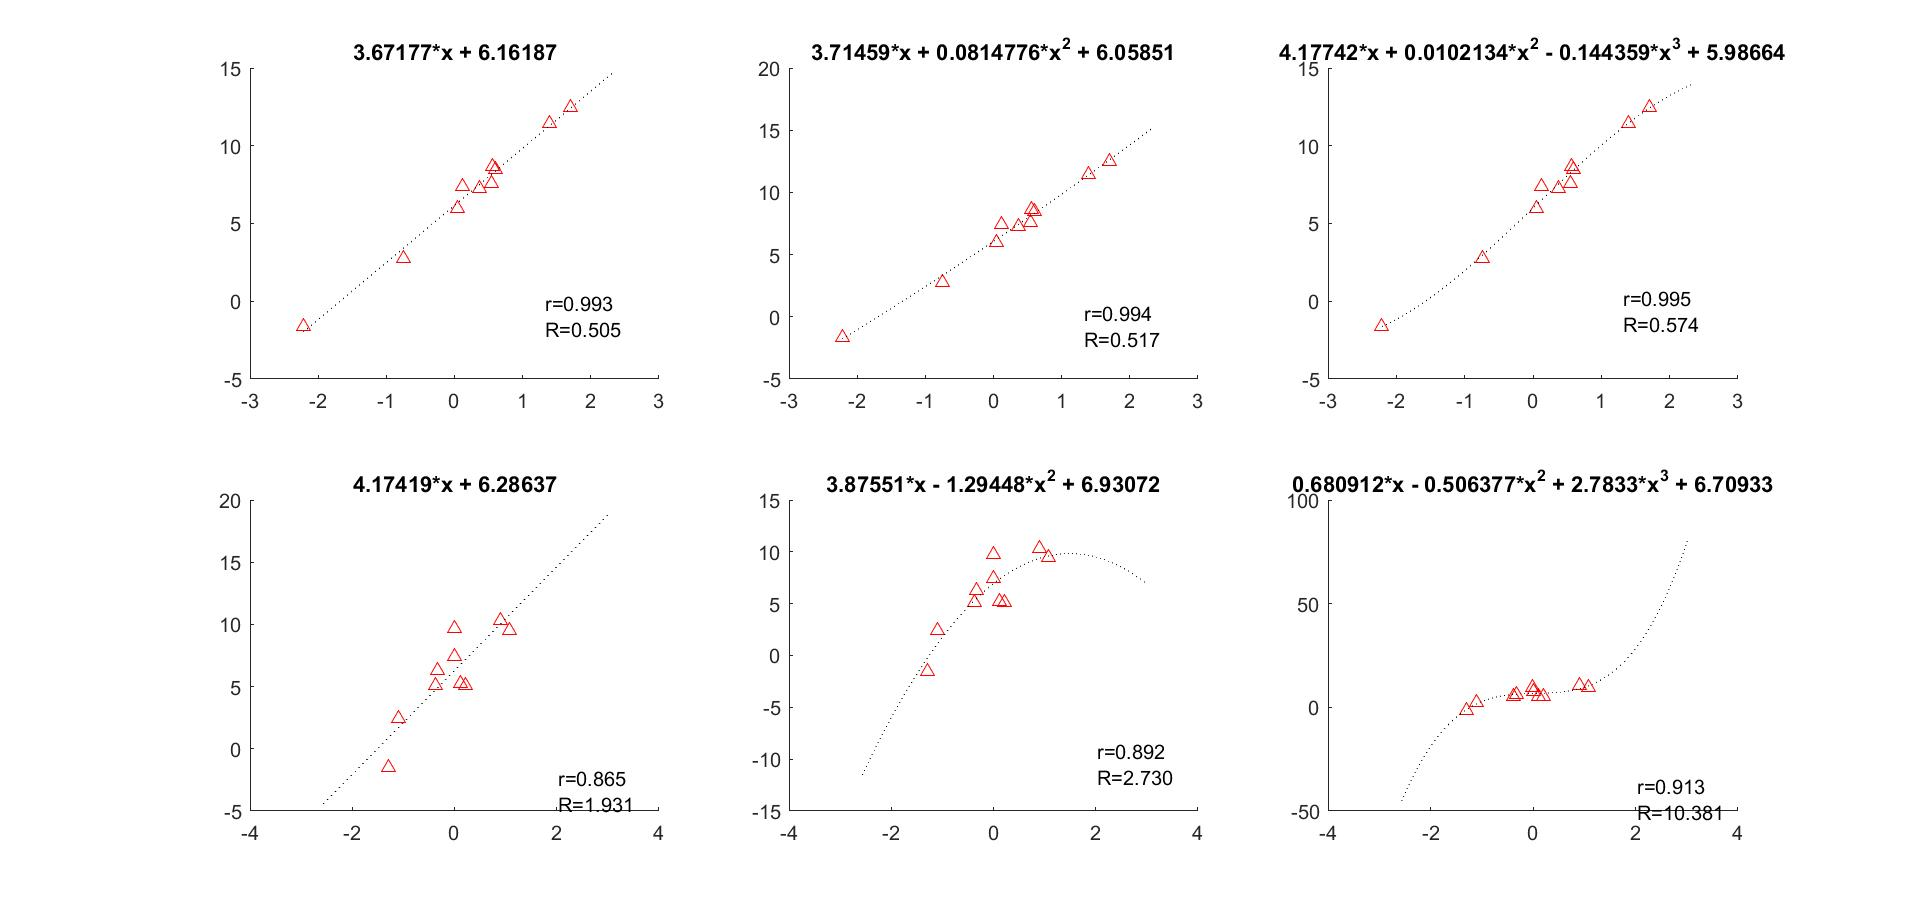
\includegraphics[width=\textwidth]{prob2/10.jpg}
\caption{10个样本点的情况}
\label{10}
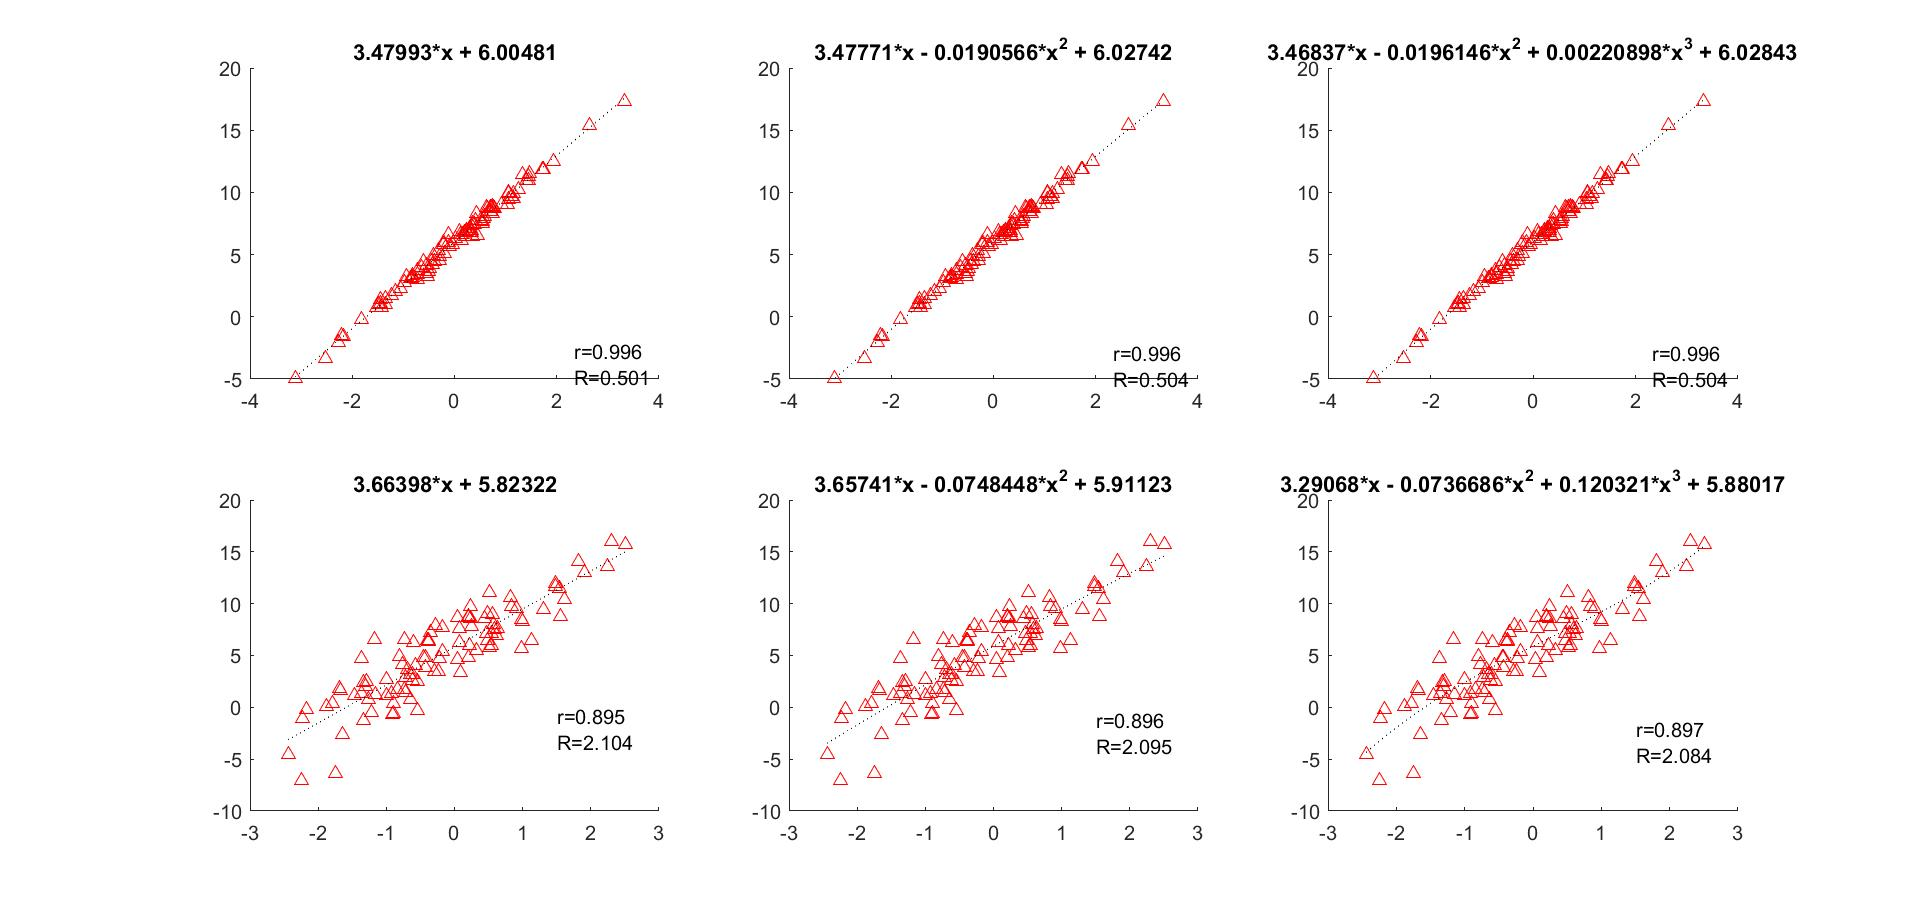
\includegraphics[width=\textwidth]{prob2/100.jpg}
\caption{100个样本点的情况}
\label{100}
\end{figure}
\section{}
经过计算得到$\hat{\theta_0}=726.0731,\hat{\theta_1}=-0.7537,\hat{\theta_2}=-161.5401,\hat{\theta_3}=61.4084$
因此(2)有$$\hat{y}=\hat{\theta_0}+110\hat{\theta_1}+3\hat{\theta_2}+\hat{\theta_3}=219.9584$$

考察交叉项可以得到$$\hat{y}=\hat{\theta_0}+\hat{\theta_1}x_1+\hat{\theta_2}x_2+\hat{\theta_3}x_3+\hat{\theta_4}x_1x_3+\hat{\theta_5}x_2x_3$$
计算得到  
$$\begin{aligned}\hat{\theta_0}=669.97,\hat{\theta_1}=-0.8563,\hat{\theta_2}=-107.602\\ \hat{\theta_3}=160.5363,\hat{\theta_4}=0.2065,\hat{\theta_5}=-98.7687\end{aligned}$$
拟合得到$\hat{y}=140$

考察$\hat{\theta_4}$对$\hat{\theta_1}$,$\hat{\theta_5}$对$\hat{\theta_2}$,当$x_3$在0和1之间变化时这些变化还是很明显的,因此认为考察交叉项有意义
\end{document}